\documentclass[border=10pt]{standalone}
\usepackage{tikz}

\begin{document}

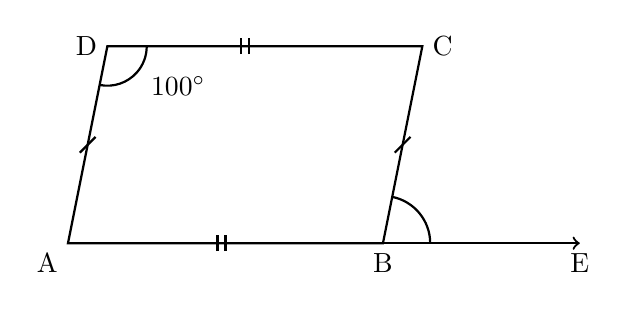
\begin{tikzpicture}[scale=1, thick]

    % 1. Define Coordinates
    \coordinate (A) at (0,0);
    \coordinate (B) at (4,0);
    \coordinate (C) at (4.5,2.5);
    \coordinate (D) at (0.5,2.5);
    \coordinate (E) at (6.5,0);

    % 2. Draw the Parallelogram and the extension ray
    \draw (A) -- (B) -- (C) -- (D) -- cycle;
    \draw[->] (B) -- (E);

    % 3. Angle at D (Interior 100 degrees)
    % Angle of segment DA is 258.69 degrees
    % We draw from the side DA to the horizontal side DC (360 degrees)
    \draw ([shift=(258.69:0.5)]D) arc (258.69:360:0.5);
    \node at (1.4,2.0) {$100^{\circ}$};

    % 4. Exterior angle at B
    % Angle of segment BC is 78.69 degrees
    \draw ([shift=(0:0.6)]B) arc (0:78.69:0.6);

    % 5. Tick Marks
    % Double ticks (Top and Bottom)
    \draw (2.2, 2.4) -- (2.2, 2.6); \draw (2.3, 2.4) -- (2.3, 2.6);
    \draw (1.9, -0.1) -- (1.9, 0.1); \draw (2.0, -0.1) -- (2.0, 0.1);

    % Single ticks (Left and Right)
    \draw (0.15, 1.15) -- (0.35, 1.35);
    \draw (4.15, 1.15) -- (4.35, 1.35);

    % 6. Labels exactly as shown in the image
    \node[below left] at (A) {A};
    \node[below] at (B) {B};
    \node[right] at (C) {C};
    \node[left] at (D) {D};
    \node[below] at (E) {E};

\end{tikzpicture}

\end{document}
